\documentclass[1p]{elsarticle_modified}
%\bibliographystyle{elsarticle-num}

%\usepackage[colorlinks]{hyperref}
%\usepackage{abbrmath_seonhwa} %\Abb, \Ascr, \Acal ,\Abf, \Afrak
\usepackage{amsfonts}
\usepackage{amssymb}
\usepackage{amsmath}
\usepackage{amsthm}
\usepackage{scalefnt}
\usepackage{amsbsy}
\usepackage{kotex}
\usepackage{caption}
\usepackage{subfig}
\usepackage{color}
\usepackage{graphicx}
\usepackage{xcolor} %% white, black, red, green, blue, cyan, magenta, yellow
\usepackage{float}
\usepackage{setspace}
\usepackage{hyperref}

\usepackage{tikz}
\usetikzlibrary{arrows}

\usepackage{multirow}
\usepackage{array} % fixed length table
\usepackage{hhline}

%%%%%%%%%%%%%%%%%%%%%
\makeatletter
\renewcommand*\env@matrix[1][\arraystretch]{%
	\edef\arraystretch{#1}%
	\hskip -\arraycolsep
	\let\@ifnextchar\new@ifnextchar
	\array{*\c@MaxMatrixCols c}}
\makeatother %https://tex.stackexchange.com/questions/14071/how-can-i-increase-the-line-spacing-in-a-matrix
%%%%%%%%%%%%%%%

\usepackage[normalem]{ulem}

\newcommand{\msout}[1]{\ifmmode\text{\sout{\ensuremath{#1}}}\else\sout{#1}\fi}
%SOURCE: \msout is \stkout macro in https://tex.stackexchange.com/questions/20609/strikeout-in-math-mode

\newcommand{\cancel}[1]{
	\ifmmode
	{\color{red}\msout{#1}}
	\else
	{\color{red}\sout{#1}}
	\fi
}

\newcommand{\add}[1]{
	{\color{blue}\uwave{#1}}
}

\newcommand{\replace}[2]{
	\ifmmode
	{\color{red}\msout{#1}}{\color{blue}\uwave{#2}}
	\else
	{\color{red}\sout{#1}}{\color{blue}\uwave{#2}}
	\fi
}

\newcommand{\Sol}{\mathcal{S}} %segment
\newcommand{\D}{D} %diagram
\newcommand{\A}{\mathcal{A}} %arc


%%%%%%%%%%%%%%%%%%%%%%%%%%%%%5 test

\def\sl{\operatorname{\textup{SL}}(2,\Cbb)}
\def\psl{\operatorname{\textup{PSL}}(2,\Cbb)}
\def\quan{\mkern 1mu \triangleright \mkern 1mu}

\theoremstyle{definition}
\newtheorem{thm}{Theorem}[section]
\newtheorem{prop}[thm]{Proposition}
\newtheorem{lem}[thm]{Lemma}
\newtheorem{ques}[thm]{Question}
\newtheorem{cor}[thm]{Corollary}
\newtheorem{defn}[thm]{Definition}
\newtheorem{exam}[thm]{Example}
\newtheorem{rmk}[thm]{Remark}
\newtheorem{alg}[thm]{Algorithm}

\newcommand{\I}{\sqrt{-1}}
\begin{document}

%\begin{frontmatter}
%
%\title{Boundary parabolic representations of knots up to 8 crossings}
%
%%% Group authors per affiliation:
%\author{Yunhi Cho} 
%\address{Department of Mathematics, University of Seoul, Seoul, Korea}
%\ead{yhcho@uos.ac.kr}
%
%
%\author{Seonhwa Kim} %\fnref{s_kim}}
%\address{Center for Geometry and Physics, Institute for Basic Science, Pohang, 37673, Korea}
%\ead{ryeona17@ibs.re.kr}
%
%\author{Hyuk Kim}
%\address{Department of Mathematical Sciences, Seoul National University, Seoul 08826, Korea}
%\ead{hyukkim@snu.ac.kr}
%
%\author{Seokbeom Yoon}
%\address{Department of Mathematical Sciences, Seoul National University, Seoul, 08826,  Korea}
%\ead{sbyoon15@snu.ac.kr}
%
%\begin{abstract}
%We find all boundary parabolic representation of knots up to 8 crossings.
%
%\end{abstract}
%\begin{keyword}
%    \MSC[2010] 57M25 
%\end{keyword}
%
%\end{frontmatter}

%\linenumbers
%\tableofcontents
%
\newcommand\colored[1]{\textcolor{white}{\rule[-0.35ex]{0.8em}{1.4ex}}\kern-0.8em\color{red} #1}%
%\newcommand\colored[1]{\textcolor{white}{ #1}\kern-2.17ex	\textcolor{white}{ #1}\kern-1.81ex	\textcolor{white}{ #1}\kern-2.15ex\color{red}#1	}

{\Large $\underline{12a_{0843}~(K12a_{0843})}$}

\setlength{\tabcolsep}{10pt}
\renewcommand{\arraystretch}{1.6}
\vspace{1cm}\begin{tabular}{m{100pt}>{\centering\arraybackslash}m{274pt}}
\multirow{5}{120pt}{
	\centering
	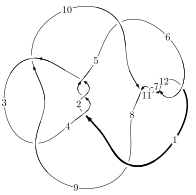
\includegraphics[width=112pt]{../../../GIT/diagram.site/Diagrams/png/1644_12a_0843.png}\\
\ \ \ A knot diagram\footnotemark}&
\allowdisplaybreaks
\textbf{Linearized knot diagam} \\
\cline{2-2}
 &
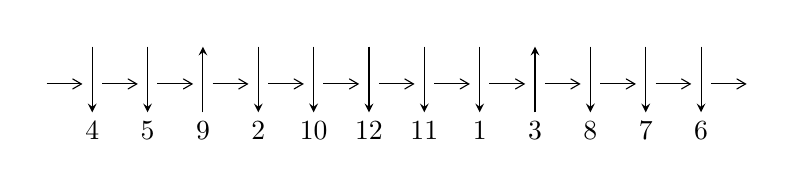
\begin{tikzpicture}[x=20pt, y=17pt]
	% nodes
	\node (C0) at (0, 0) {};
	\node (C1) at (1, 0) {};
	\node (C1U) at (1, +1) {};
	\node (C1D) at (1, -1) {4};

	\node (C2) at (2, 0) {};
	\node (C2U) at (2, +1) {};
	\node (C2D) at (2, -1) {5};

	\node (C3) at (3, 0) {};
	\node (C3U) at (3, +1) {};
	\node (C3D) at (3, -1) {9};

	\node (C4) at (4, 0) {};
	\node (C4U) at (4, +1) {};
	\node (C4D) at (4, -1) {2};

	\node (C5) at (5, 0) {};
	\node (C5U) at (5, +1) {};
	\node (C5D) at (5, -1) {10};

	\node (C6) at (6, 0) {};
	\node (C6U) at (6, +1) {};
	\node (C6D) at (6, -1) {12};

	\node (C7) at (7, 0) {};
	\node (C7U) at (7, +1) {};
	\node (C7D) at (7, -1) {11};

	\node (C8) at (8, 0) {};
	\node (C8U) at (8, +1) {};
	\node (C8D) at (8, -1) {1};

	\node (C9) at (9, 0) {};
	\node (C9U) at (9, +1) {};
	\node (C9D) at (9, -1) {3};

	\node (C10) at (10, 0) {};
	\node (C10U) at (10, +1) {};
	\node (C10D) at (10, -1) {8};

	\node (C11) at (11, 0) {};
	\node (C11U) at (11, +1) {};
	\node (C11D) at (11, -1) {7};

	\node (C12) at (12, 0) {};
	\node (C12U) at (12, +1) {};
	\node (C12D) at (12, -1) {6};
	\node (C13) at (13, 0) {};

	% arrows
	\draw[->,>={angle 60}]
	(C0) edge (C1) (C1) edge (C2) (C2) edge (C3) (C3) edge (C4) (C4) edge (C5) (C5) edge (C6) (C6) edge (C7) (C7) edge (C8) (C8) edge (C9) (C9) edge (C10) (C10) edge (C11) (C11) edge (C12) (C12) edge (C13) ;	\draw[->,>=stealth]
	(C1U) edge (C1D) (C2U) edge (C2D) (C3D) edge (C3U) (C4U) edge (C4D) (C5U) edge (C5D) (C6U) edge (C6D) (C7U) edge (C7D) (C8U) edge (C8D) (C9D) edge (C9U) (C10U) edge (C10D) (C11U) edge (C11D) (C12U) edge (C12D) ;
	\end{tikzpicture} \\
\hhline{~~} \\& 
\textbf{Solving Sequence} \\ \cline{2-2} 
 &
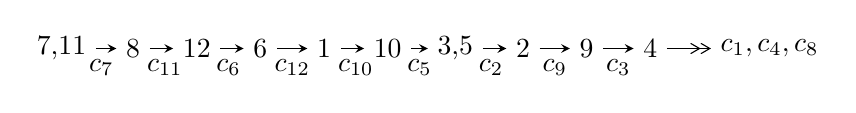
\begin{tikzpicture}[x=23pt, y=7pt]
	% node
	\node (A0) at (-1/8, 0) {7,11};
	\node (A1) at (1, 0) {8};
	\node (A2) at (2, 0) {12};
	\node (A3) at (3, 0) {6};
	\node (A4) at (4, 0) {1};
	\node (A5) at (5, 0) {10};
	\node (A6) at (97/16, 0) {3,5};
	\node (A7) at (57/8, 0) {2};
	\node (A8) at (65/8, 0) {9};
	\node (A9) at (73/8, 0) {4};
	\node (C1) at (1/2, -1) {$c_{7}$};
	\node (C2) at (3/2, -1) {$c_{11}$};
	\node (C3) at (5/2, -1) {$c_{6}$};
	\node (C4) at (7/2, -1) {$c_{12}$};
	\node (C5) at (9/2, -1) {$c_{10}$};
	\node (C6) at (11/2, -1) {$c_{5}$};
	\node (C7) at (53/8, -1) {$c_{2}$};
	\node (C8) at (61/8, -1) {$c_{9}$};
	\node (C9) at (69/8, -1) {$c_{3}$};
	\node (A10) at (11, 0) {$c_{1},c_{4},c_{8}$};

	% edge
	\draw[->,>=stealth]	
	(A0) edge (A1) (A1) edge (A2) (A2) edge (A3) (A3) edge (A4) (A4) edge (A5) (A5) edge (A6) (A6) edge (A7) (A7) edge (A8) (A8) edge (A9) ;
	\draw[->>,>={angle 60}]	
	(A9) edge (A10);
\end{tikzpicture} \\ 

\end{tabular} \\

\footnotetext{
The image of knot diagram is generated by the software ``\textbf{Draw programme}" developed by Andrew Bartholomew(\url{http://www.layer8.co.uk/maths/draw/index.htm\#Running-draw}), where we modified some parts for our purpose(\url{https://github.com/CATsTAILs/LinksPainter}).
}\phantom \\ \newline 
\centering \textbf{Ideals for irreducible components\footnotemark of $X_{\text{par}}$} 
 
\begin{align*}
I^u_{1}&=\langle 
u^{45}+26 u^{43}+\cdots+b-1,\;- u^{46}-3 u^{45}+\cdots+a-2,\;u^{47}+2 u^{46}+\cdots+2 u+1\rangle \\
I^u_{2}&=\langle 
u^2+b- u+1,\;u^4- u^3+3 u^2+a-2 u+1,\;u^5- u^4+4 u^3-3 u^2+3 u-1\rangle \\
\\
\end{align*}
\raggedright * 2 irreducible components of $\dim_{\mathbb{C}}=0$, with total 52 representations.\\
\footnotetext{All coefficients of polynomials are rational numbers. But the coefficients are sometimes approximated in decimal forms when there is not enough margin.}
\newpage
\renewcommand{\arraystretch}{1}
\centering \section*{I. $I^u_{1}= \langle u^{45}+26 u^{43}+\cdots+b-1,\;- u^{46}-3 u^{45}+\cdots+a-2,\;u^{47}+2 u^{46}+\cdots+2 u+1 \rangle$}
\flushleft \textbf{(i) Arc colorings}\\
\begin{tabular}{m{7pt} m{180pt} m{7pt} m{180pt} }
\flushright $a_{7}=$&$\begin{pmatrix}1\\0\end{pmatrix}$ \\
\flushright $a_{11}=$&$\begin{pmatrix}0\\u\end{pmatrix}$ \\
\flushright $a_{8}=$&$\begin{pmatrix}1\\u^2\end{pmatrix}$ \\
\flushright $a_{12}=$&$\begin{pmatrix}- u\\u\end{pmatrix}$ \\
\flushright $a_{6}=$&$\begin{pmatrix}u^2+1\\- u^2\end{pmatrix}$ \\
\flushright $a_{1}=$&$\begin{pmatrix}- u^3-2 u\\u^3+u\end{pmatrix}$ \\
\flushright $a_{10}=$&$\begin{pmatrix}u\\u^3+u\end{pmatrix}$ \\
\flushright $a_{3}=$&$\begin{pmatrix}u^{46}+3 u^{45}+\cdots-5 u+2\\- u^{45}-26 u^{43}+\cdots- u+1\end{pmatrix}$ \\
\flushright $a_{5}=$&$\begin{pmatrix}- u^6-3 u^4+1\\- u^8-4 u^6-4 u^4-2 u^2\end{pmatrix}$ \\
\flushright $a_{2}=$&$\begin{pmatrix}u^{46}+2 u^{45}+\cdots-7 u+2\\u^{44}+2 u^{43}+\cdots- u^2+1\end{pmatrix}$ \\
\flushright $a_{9}=$&$\begin{pmatrix}- u^8-5 u^6-7 u^4-2 u^2+1\\u^8+4 u^6+4 u^4+2 u^2\end{pmatrix}$ \\
\flushright $a_{4}=$&$\begin{pmatrix}u^{46}+u^{45}+\cdots-7 u+1\\u^{45}+2 u^{44}+\cdots+19 u^3+1\end{pmatrix}$\\&\end{tabular}
\flushleft \textbf{(ii) Obstruction class $= -1$}\\~\\
\flushleft \textbf{(iii) Cusp Shapes $= u^{46}+2 u^{45}+\cdots-3 u-2$}\\~\\
\newpage\renewcommand{\arraystretch}{1}
\flushleft \textbf{(iv) u-Polynomials at the component}\newline \\
\begin{tabular}{m{50pt}|m{274pt}}
Crossings & \hspace{64pt}u-Polynomials at each crossing \\
\hline $$\begin{aligned}c_{1},c_{2},c_{4}\end{aligned}$$&$\begin{aligned}
&u^{47}-6 u^{46}+\cdots+4 u-1
\end{aligned}$\\
\hline $$\begin{aligned}c_{3},c_{9}\end{aligned}$$&$\begin{aligned}
&u^{47}- u^{46}+\cdots-64 u-32
\end{aligned}$\\
\hline $$\begin{aligned}c_{5},c_{8}\end{aligned}$$&$\begin{aligned}
&u^{47}-2 u^{46}+\cdots+160 u-100
\end{aligned}$\\
\hline $$\begin{aligned}c_{6},c_{7},c_{10}\\c_{11},c_{12}\end{aligned}$$&$\begin{aligned}
&u^{47}-2 u^{46}+\cdots+2 u-1
\end{aligned}$\\
\hline
\end{tabular}\\~\\
\newpage\renewcommand{\arraystretch}{1}
\flushleft \textbf{(v) Riley Polynomials at the component}\newline \\
\begin{tabular}{m{50pt}|m{274pt}}
Crossings & \hspace{64pt}Riley Polynomials at each crossing \\
\hline $$\begin{aligned}c_{1},c_{2},c_{4}\end{aligned}$$&$\begin{aligned}
&y^{47}-48 y^{46}+\cdots+28 y-1
\end{aligned}$\\
\hline $$\begin{aligned}c_{3},c_{9}\end{aligned}$$&$\begin{aligned}
&y^{47}+33 y^{46}+\cdots+3584 y-1024
\end{aligned}$\\
\hline $$\begin{aligned}c_{5},c_{8}\end{aligned}$$&$\begin{aligned}
&y^{47}-36 y^{46}+\cdots+55800 y-10000
\end{aligned}$\\
\hline $$\begin{aligned}c_{6},c_{7},c_{10}\\c_{11},c_{12}\end{aligned}$$&$\begin{aligned}
&y^{47}+60 y^{46}+\cdots+18 y-1
\end{aligned}$\\
\hline
\end{tabular}\\~\\
\newpage\flushleft \textbf{(vi) Complex Volumes and Cusp Shapes}
$$\begin{array}{c|c|c}  
\text{Solutions to }I^u_{1}& \I (\text{vol} + \sqrt{-1}CS) & \text{Cusp shape}\\
 \hline 
\begin{aligned}
u &= -0.413508 + 0.910925 I \\
a &= -1.83324 - 1.08728 I \\
b &= -0.378490 - 0.145011 I\end{aligned}
 & -8.75070 + 10.08960 I & -10.18236 - 7.10316 I \\ \hline\begin{aligned}
u &= -0.413508 - 0.910925 I \\
a &= -1.83324 + 1.08728 I \\
b &= -0.378490 + 0.145011 I\end{aligned}
 & -8.75070 - 10.08960 I & -10.18236 + 7.10316 I \\ \hline\begin{aligned}
u &= -0.381689 + 0.871051 I \\
a &= \phantom{-}2.02691 + 1.16470 I \\
b &= \phantom{-}0.497884 - 0.080589 I\end{aligned}
 & -2.05630 + 5.96873 I & -8.18293 - 7.13665 I \\ \hline\begin{aligned}
u &= -0.381689 - 0.871051 I \\
a &= \phantom{-}2.02691 - 1.16470 I \\
b &= \phantom{-}0.497884 + 0.080589 I\end{aligned}
 & -2.05630 - 5.96873 I & -8.18293 + 7.13665 I \\ \hline\begin{aligned}
u &= \phantom{-}0.091071 + 0.931262 I \\
a &= \phantom{-}0.711455 - 0.425911 I \\
b &= -0.488416 - 0.498587 I\end{aligned}
 & \phantom{-}3.10179 - 1.86671 I & -0.52311 + 5.01743 I \\ \hline\begin{aligned}
u &= \phantom{-}0.091071 - 0.931262 I \\
a &= \phantom{-}0.711455 + 0.425911 I \\
b &= -0.488416 + 0.498587 I\end{aligned}
 & \phantom{-}3.10179 + 1.86671 I & -0.52311 - 5.01743 I \\ \hline\begin{aligned}
u &= \phantom{-}0.192703 + 1.050590 I \\
a &= -0.491605 + 0.630434 I \\
b &= \phantom{-}0.819514 + 0.152813 I\end{aligned}
 & -1.81566 - 3.80529 I & -8.08850 + 4.35592 I \\ \hline\begin{aligned}
u &= \phantom{-}0.192703 - 1.050590 I \\
a &= -0.491605 - 0.630434 I \\
b &= \phantom{-}0.819514 - 0.152813 I\end{aligned}
 & -1.81566 + 3.80529 I & -8.08850 - 4.35592 I \\ \hline\begin{aligned}
u &= \phantom{-}0.386775 + 0.839886 I \\
a &= \phantom{-}0.354292 + 0.843743 I \\
b &= \phantom{-}0.287734 - 0.602113 I\end{aligned}
 & -4.41584 - 3.34895 I & -9.57199 + 4.15022 I \\ \hline\begin{aligned}
u &= \phantom{-}0.386775 - 0.839886 I \\
a &= \phantom{-}0.354292 - 0.843743 I \\
b &= \phantom{-}0.287734 + 0.602113 I\end{aligned}
 & -4.41584 + 3.34895 I & -9.57199 - 4.15022 I\\
 \hline 
 \end{array}$$\newpage$$\begin{array}{c|c|c}  
\text{Solutions to }I^u_{1}& \I (\text{vol} + \sqrt{-1}CS) & \text{Cusp shape}\\
 \hline 
\begin{aligned}
u &= \phantom{-}0.275185 + 0.865499 I \\
a &= -0.224202 - 0.422215 I \\
b &= -0.175658 + 0.313273 I\end{aligned}
 & \phantom{-}1.41842 - 2.55289 I & -1.19798 + 4.60383 I \\ \hline\begin{aligned}
u &= \phantom{-}0.275185 - 0.865499 I \\
a &= -0.224202 + 0.422215 I \\
b &= -0.175658 - 0.313273 I\end{aligned}
 & \phantom{-}1.41842 + 2.55289 I & -1.19798 - 4.60383 I \\ \hline\begin{aligned}
u &= -0.376433 + 0.803567 I \\
a &= -2.17677 - 0.95906 I \\
b &= -0.372360 + 0.375511 I\end{aligned}
 & -2.47676 + 0.64455 I & -9.45745 - 1.20852 I \\ \hline\begin{aligned}
u &= -0.376433 - 0.803567 I \\
a &= -2.17677 + 0.95906 I \\
b &= -0.372360 - 0.375511 I\end{aligned}
 & -2.47676 - 0.64455 I & -9.45745 + 1.20852 I \\ \hline\begin{aligned}
u &= -0.441065 + 0.749468 I \\
a &= \phantom{-}2.04675 + 0.85956 I \\
b &= \phantom{-}0.100717 - 0.418593 I\end{aligned}
 & -9.72112 - 2.90941 I & -11.56361 - 0.62182 I \\ \hline\begin{aligned}
u &= -0.441065 - 0.749468 I \\
a &= \phantom{-}2.04675 - 0.85956 I \\
b &= \phantom{-}0.100717 + 0.418593 I\end{aligned}
 & -9.72112 + 2.90941 I & -11.56361 + 0.62182 I \\ \hline\begin{aligned}
u &= -0.064336 + 0.822622 I \\
a &= -1.48802 + 0.46619 I \\
b &= \phantom{-}0.238982 + 0.908240 I\end{aligned}
 & \phantom{-}0.328476 + 0.959018 I & -5.90793 + 0.74635 I \\ \hline\begin{aligned}
u &= -0.064336 - 0.822622 I \\
a &= -1.48802 - 0.46619 I \\
b &= \phantom{-}0.238982 - 0.908240 I\end{aligned}
 & \phantom{-}0.328476 - 0.959018 I & -5.90793 - 0.74635 I \\ \hline\begin{aligned}
u &= -0.638824 + 0.074996 I \\
a &= -0.421838 - 0.513599 I \\
b &= -0.04958 + 1.70077 I\end{aligned}
 & -11.75550 + 6.54260 I & -15.0022 - 4.1132 I \\ \hline\begin{aligned}
u &= -0.638824 - 0.074996 I \\
a &= -0.421838 + 0.513599 I \\
b &= -0.04958 - 1.70077 I\end{aligned}
 & -11.75550 - 6.54260 I & -15.0022 + 4.1132 I\\
 \hline 
 \end{array}$$\newpage$$\begin{array}{c|c|c}  
\text{Solutions to }I^u_{1}& \I (\text{vol} + \sqrt{-1}CS) & \text{Cusp shape}\\
 \hline 
\begin{aligned}
u &= \phantom{-}0.602974\phantom{ +0.000000I} \\
a &= \phantom{-}1.18447\phantom{ +0.000000I} \\
b &= -0.503637\phantom{ +0.000000I}\end{aligned}
 & -6.95614\phantom{ +0.000000I} & -14.4200\phantom{ +0.000000I} \\ \hline\begin{aligned}
u &= -0.596607 + 0.032355 I \\
a &= \phantom{-}0.220109 + 0.214041 I \\
b &= \phantom{-}0.05568 - 1.78658 I\end{aligned}
 & -4.79872 + 2.65777 I & -13.67344 - 3.52824 I \\ \hline\begin{aligned}
u &= -0.596607 - 0.032355 I \\
a &= \phantom{-}0.220109 - 0.214041 I \\
b &= \phantom{-}0.05568 + 1.78658 I\end{aligned}
 & -4.79872 - 2.65777 I & -13.67344 + 3.52824 I \\ \hline\begin{aligned}
u &= \phantom{-}0.474154 + 0.347428 I \\
a &= \phantom{-}1.099760 + 0.840634 I \\
b &= -0.249987 - 0.545071 I\end{aligned}
 & -6.24028 - 1.59922 I & -13.28615 + 4.03816 I \\ \hline\begin{aligned}
u &= \phantom{-}0.474154 - 0.347428 I \\
a &= \phantom{-}1.099760 - 0.840634 I \\
b &= -0.249987 + 0.545071 I\end{aligned}
 & -6.24028 + 1.59922 I & -13.28615 - 4.03816 I \\ \hline\begin{aligned}
u &= \phantom{-}0.473616\phantom{ +0.000000I} \\
a &= -0.668057\phantom{ +0.000000I} \\
b &= \phantom{-}0.235856\phantom{ +0.000000I}\end{aligned}
 & -1.20734\phantom{ +0.000000I} & -8.21660\phantom{ +0.000000I} \\ \hline\begin{aligned}
u &= -0.09345 + 1.61990 I \\
a &= -1.84799 - 0.75382 I \\
b &= \phantom{-}3.72034 + 1.96860 I\end{aligned}
 & -1.65071 - 1.00207 I & \phantom{-0.000000 } 0 \\ \hline\begin{aligned}
u &= -0.09345 - 1.61990 I \\
a &= -1.84799 + 0.75382 I \\
b &= \phantom{-}3.72034 - 1.96860 I\end{aligned}
 & -1.65071 + 1.00207 I & \phantom{-0.000000 } 0 \\ \hline\begin{aligned}
u &= -0.08668 + 1.65706 I \\
a &= \phantom{-}2.61073 + 1.11521 I \\
b &= -4.96661 - 2.65420 I\end{aligned}
 & \phantom{-}6.07762 + 2.32488 I & \phantom{-0.000000 } 0 \\ \hline\begin{aligned}
u &= -0.08668 - 1.65706 I \\
a &= \phantom{-}2.61073 - 1.11521 I \\
b &= -4.96661 + 2.65420 I\end{aligned}
 & \phantom{-}6.07762 - 2.32488 I & \phantom{-0.000000 } 0\\
 \hline 
 \end{array}$$\newpage$$\begin{array}{c|c|c}  
\text{Solutions to }I^u_{1}& \I (\text{vol} + \sqrt{-1}CS) & \text{Cusp shape}\\
 \hline 
\begin{aligned}
u &= \phantom{-}0.09573 + 1.66580 I \\
a &= -1.009190 - 0.039969 I \\
b &= \phantom{-}1.63623 + 0.52270 I\end{aligned}
 & \phantom{-}4.30233 - 5.15506 I & \phantom{-0.000000 } 0 \\ \hline\begin{aligned}
u &= \phantom{-}0.09573 - 1.66580 I \\
a &= -1.009190 + 0.039969 I \\
b &= \phantom{-}1.63623 - 0.52270 I\end{aligned}
 & \phantom{-}4.30233 + 5.15506 I & \phantom{-0.000000 } 0 \\ \hline\begin{aligned}
u &= \phantom{-}0.238719 + 0.226721 I \\
a &= -1.01393 - 1.12454 I \\
b &= \phantom{-}0.038509 + 0.406266 I\end{aligned}
 & -0.387281 - 0.808831 I & -8.67312 + 8.42283 I \\ \hline\begin{aligned}
u &= \phantom{-}0.238719 - 0.226721 I \\
a &= -1.01393 + 1.12454 I \\
b &= \phantom{-}0.038509 - 0.406266 I\end{aligned}
 & -0.387281 + 0.808831 I & -8.67312 - 8.42283 I \\ \hline\begin{aligned}
u &= -0.01112 + 1.67312 I \\
a &= \phantom{-}1.51780 - 1.37183 I \\
b &= -3.19718 + 2.02255 I\end{aligned}
 & \phantom{-}9.18863 + 1.20864 I & \phantom{-0.000000 } 0 \\ \hline\begin{aligned}
u &= -0.01112 - 1.67312 I \\
a &= \phantom{-}1.51780 + 1.37183 I \\
b &= -3.19718 - 2.02255 I\end{aligned}
 & \phantom{-}9.18863 - 1.20864 I & \phantom{-0.000000 } 0 \\ \hline\begin{aligned}
u &= -0.09778 + 1.67602 I \\
a &= -2.52969 - 1.85960 I \\
b &= \phantom{-}4.67873 + 3.90951 I\end{aligned}
 & \phantom{-}6.83164 + 7.79802 I & \phantom{-0.000000 } 0 \\ \hline\begin{aligned}
u &= -0.09778 - 1.67602 I \\
a &= -2.52969 + 1.85960 I \\
b &= \phantom{-}4.67873 - 3.90951 I\end{aligned}
 & \phantom{-}6.83164 - 7.79802 I & \phantom{-0.000000 } 0 \\ \hline\begin{aligned}
u &= \phantom{-}0.06732 + 1.68247 I \\
a &= \phantom{-}0.599873 - 0.006463 I \\
b &= -1.007440 - 0.229685 I\end{aligned}
 & \phantom{-}10.40890 - 3.84665 I & \phantom{-0.000000 } 0 \\ \hline\begin{aligned}
u &= \phantom{-}0.06732 - 1.68247 I \\
a &= \phantom{-}0.599873 + 0.006463 I \\
b &= -1.007440 + 0.229685 I\end{aligned}
 & \phantom{-}10.40890 + 3.84665 I & \phantom{-0.000000 } 0\\
 \hline 
 \end{array}$$\newpage$$\begin{array}{c|c|c}  
\text{Solutions to }I^u_{1}& \I (\text{vol} + \sqrt{-1}CS) & \text{Cusp shape}\\
 \hline 
\begin{aligned}
u &= -0.11098 + 1.68676 I \\
a &= \phantom{-}2.12470 + 2.11421 I \\
b &= -3.92124 - 4.22596 I\end{aligned}
 & \phantom{-}0.30937 + 12.13810 I & \phantom{-0.000000 } 0 \\ \hline\begin{aligned}
u &= -0.11098 - 1.68676 I \\
a &= \phantom{-}2.12470 - 2.11421 I \\
b &= -3.92124 + 4.22596 I\end{aligned}
 & \phantom{-}0.30937 - 12.13810 I & \phantom{-0.000000 } 0 \\ \hline\begin{aligned}
u &= \phantom{-}0.02004 + 1.69490 I \\
a &= -0.497803 + 1.204650 I \\
b &= \phantom{-}1.25861 - 1.93145 I\end{aligned}
 & \phantom{-}12.42340 - 2.28034 I & \phantom{-0.000000 } 0 \\ \hline\begin{aligned}
u &= \phantom{-}0.02004 - 1.69490 I \\
a &= -0.497803 - 1.204650 I \\
b &= \phantom{-}1.25861 + 1.93145 I\end{aligned}
 & \phantom{-}12.42340 + 2.28034 I & \phantom{-0.000000 } 0 \\ \hline\begin{aligned}
u &= \phantom{-}0.04372 + 1.72277 I \\
a &= -0.332562 - 1.108820 I \\
b &= \phantom{-}0.20612 + 1.95580 I\end{aligned}
 & \phantom{-}8.05569 - 4.72882 I & \phantom{-0.000000 } 0 \\ \hline\begin{aligned}
u &= \phantom{-}0.04372 - 1.72277 I \\
a &= -0.332562 + 1.108820 I \\
b &= \phantom{-}0.20612 - 1.95580 I\end{aligned}
 & \phantom{-}8.05569 + 4.72882 I & \phantom{-0.000000 } 0 \\ \hline\begin{aligned}
u &= -0.222465\phantom{ +0.000000I} \\
a &= \phantom{-}2.59250\phantom{ +0.000000I} \\
b &= \phantom{-}0.803601\phantom{ +0.000000I}\end{aligned}
 & -2.01148\phantom{ +0.000000I} & -1.29870\phantom{ +0.000000I}\\
 \hline 
 \end{array}$$\newpage\newpage\renewcommand{\arraystretch}{1}
\centering \section*{II. $I^u_{2}= \langle u^2+b- u+1,\;u^4- u^3+3 u^2+a-2 u+1,\;u^5- u^4+4 u^3-3 u^2+3 u-1 \rangle$}
\flushleft \textbf{(i) Arc colorings}\\
\begin{tabular}{m{7pt} m{180pt} m{7pt} m{180pt} }
\flushright $a_{7}=$&$\begin{pmatrix}1\\0\end{pmatrix}$ \\
\flushright $a_{11}=$&$\begin{pmatrix}0\\u\end{pmatrix}$ \\
\flushright $a_{8}=$&$\begin{pmatrix}1\\u^2\end{pmatrix}$ \\
\flushright $a_{12}=$&$\begin{pmatrix}- u\\u\end{pmatrix}$ \\
\flushright $a_{6}=$&$\begin{pmatrix}u^2+1\\- u^2\end{pmatrix}$ \\
\flushright $a_{1}=$&$\begin{pmatrix}- u^3-2 u\\u^3+u\end{pmatrix}$ \\
\flushright $a_{10}=$&$\begin{pmatrix}u\\u^3+u\end{pmatrix}$ \\
\flushright $a_{3}=$&$\begin{pmatrix}- u^4+u^3-3 u^2+2 u-1\\- u^2+u-1\end{pmatrix}$ \\
\flushright $a_{5}=$&$\begin{pmatrix}u^3+2 u\\- u^3- u\end{pmatrix}$ \\
\flushright $a_{2}=$&$\begin{pmatrix}- u^4-3 u^2-1\\u^3- u^2+2 u-1\end{pmatrix}$ \\
\flushright $a_{9}=$&$\begin{pmatrix}u\\u^3+u\end{pmatrix}$ \\
\flushright $a_{4}=$&$\begin{pmatrix}- u^4+u^3-3 u^2+2 u-1\\- u^2+u-1\end{pmatrix}$\\&\end{tabular}
\flushleft \textbf{(ii) Obstruction class $= 1$}\\~\\
\flushleft \textbf{(iii) Cusp Shapes $= -5 u^4+5 u^3-20 u^2+14 u-21$}\\~\\
\newpage\renewcommand{\arraystretch}{1}
\flushleft \textbf{(iv) u-Polynomials at the component}\newline \\
\begin{tabular}{m{50pt}|m{274pt}}
Crossings & \hspace{64pt}u-Polynomials at each crossing \\
\hline $$\begin{aligned}c_{1},c_{2}\end{aligned}$$&$\begin{aligned}
&(u-1)^5
\end{aligned}$\\
\hline $$\begin{aligned}c_{3},c_{9}\end{aligned}$$&$\begin{aligned}
&u^5
\end{aligned}$\\
\hline $$\begin{aligned}c_{4}\end{aligned}$$&$\begin{aligned}
&(u+1)^5
\end{aligned}$\\
\hline $$\begin{aligned}c_{5},c_{8}\end{aligned}$$&$\begin{aligned}
&u^5- u^4+u^2+u-1
\end{aligned}$\\
\hline $$\begin{aligned}c_{6},c_{7}\end{aligned}$$&$\begin{aligned}
&u^5- u^4+4 u^3-3 u^2+3 u-1
\end{aligned}$\\
\hline $$\begin{aligned}c_{10},c_{11},c_{12}\end{aligned}$$&$\begin{aligned}
&u^5+u^4+4 u^3+3 u^2+3 u+1
\end{aligned}$\\
\hline
\end{tabular}\\~\\
\newpage\renewcommand{\arraystretch}{1}
\flushleft \textbf{(v) Riley Polynomials at the component}\newline \\
\begin{tabular}{m{50pt}|m{274pt}}
Crossings & \hspace{64pt}Riley Polynomials at each crossing \\
\hline $$\begin{aligned}c_{1},c_{2},c_{4}\end{aligned}$$&$\begin{aligned}
&(y-1)^5
\end{aligned}$\\
\hline $$\begin{aligned}c_{3},c_{9}\end{aligned}$$&$\begin{aligned}
&y^5
\end{aligned}$\\
\hline $$\begin{aligned}c_{5},c_{8}\end{aligned}$$&$\begin{aligned}
&y^5- y^4+4 y^3-3 y^2+3 y-1
\end{aligned}$\\
\hline $$\begin{aligned}c_{6},c_{7},c_{10}\\c_{11},c_{12}\end{aligned}$$&$\begin{aligned}
&y^5+7 y^4+16 y^3+13 y^2+3 y-1
\end{aligned}$\\
\hline
\end{tabular}\\~\\
\newpage\flushleft \textbf{(vi) Complex Volumes and Cusp Shapes}
$$\begin{array}{c|c|c}  
\text{Solutions to }I^u_{2}& \I (\text{vol} + \sqrt{-1}CS) & \text{Cusp shape}\\
 \hline 
\begin{aligned}
u &= \phantom{-}0.233677 + 0.885557 I \\
a &= \phantom{-}0.758138 + 0.584034 I \\
b &= -0.036717 + 0.471689 I\end{aligned}
 & \phantom{-}0.17487 - 2.21397 I & -7.62657 + 4.39306 I \\ \hline\begin{aligned}
u &= \phantom{-}0.233677 - 0.885557 I \\
a &= \phantom{-}0.758138 - 0.584034 I \\
b &= -0.036717 - 0.471689 I\end{aligned}
 & \phantom{-}0.17487 + 2.21397 I & -7.62657 - 4.39306 I \\ \hline\begin{aligned}
u &= \phantom{-}0.416284\phantom{ +0.000000I} \\
a &= -0.645200\phantom{ +0.000000I} \\
b &= -0.757008\phantom{ +0.000000I}\end{aligned}
 & -2.52712\phantom{ +0.000000I} & -18.4270\phantom{ +0.000000I} \\ \hline\begin{aligned}
u &= \phantom{-}0.05818 + 1.69128 I \\
a &= -0.935538 - 0.903908 I \\
b &= \phantom{-}1.91522 + 1.49448 I\end{aligned}
 & \phantom{-}9.31336 - 3.33174 I & -6.15976 + 1.26157 I \\ \hline\begin{aligned}
u &= \phantom{-}0.05818 - 1.69128 I \\
a &= -0.935538 + 0.903908 I \\
b &= \phantom{-}1.91522 - 1.49448 I\end{aligned}
 & \phantom{-}9.31336 + 3.33174 I & -6.15976 - 1.26157 I\\
 \hline 
 \end{array}$$\newpage
\newpage\renewcommand{\arraystretch}{1}
\centering \section*{ III. u-Polynomials}
\begin{tabular}{m{50pt}|m{274pt}}
Crossings & \hspace{64pt}u-Polynomials at each crossing \\
\hline $$\begin{aligned}c_{1},c_{2}\end{aligned}$$&$\begin{aligned}
&((u-1)^5)(u^{47}-6 u^{46}+\cdots+4 u-1)
\end{aligned}$\\
\hline $$\begin{aligned}c_{3},c_{9}\end{aligned}$$&$\begin{aligned}
&u^5(u^{47}- u^{46}+\cdots-64 u-32)
\end{aligned}$\\
\hline $$\begin{aligned}c_{4}\end{aligned}$$&$\begin{aligned}
&((u+1)^5)(u^{47}-6 u^{46}+\cdots+4 u-1)
\end{aligned}$\\
\hline $$\begin{aligned}c_{5},c_{8}\end{aligned}$$&$\begin{aligned}
&(u^5- u^4+u^2+u-1)(u^{47}-2 u^{46}+\cdots+160 u-100)
\end{aligned}$\\
\hline $$\begin{aligned}c_{6},c_{7}\end{aligned}$$&$\begin{aligned}
&(u^5- u^4+4 u^3-3 u^2+3 u-1)(u^{47}-2 u^{46}+\cdots+2 u-1)
\end{aligned}$\\
\hline $$\begin{aligned}c_{10},c_{11},c_{12}\end{aligned}$$&$\begin{aligned}
&(u^5+u^4+4 u^3+3 u^2+3 u+1)(u^{47}-2 u^{46}+\cdots+2 u-1)
\end{aligned}$\\
\hline
\end{tabular}\newpage\renewcommand{\arraystretch}{1}
\centering \section*{ IV. Riley Polynomials}
\begin{tabular}{m{50pt}|m{274pt}}
Crossings & \hspace{64pt}Riley Polynomials at each crossing \\
\hline $$\begin{aligned}c_{1},c_{2},c_{4}\end{aligned}$$&$\begin{aligned}
&((y-1)^5)(y^{47}-48 y^{46}+\cdots+28 y-1)
\end{aligned}$\\
\hline $$\begin{aligned}c_{3},c_{9}\end{aligned}$$&$\begin{aligned}
&y^5(y^{47}+33 y^{46}+\cdots+3584 y-1024)
\end{aligned}$\\
\hline $$\begin{aligned}c_{5},c_{8}\end{aligned}$$&$\begin{aligned}
&(y^5- y^4+4 y^3-3 y^2+3 y-1)(y^{47}-36 y^{46}+\cdots+55800 y-10000)
\end{aligned}$\\
\hline $$\begin{aligned}c_{6},c_{7},c_{10}\\c_{11},c_{12}\end{aligned}$$&$\begin{aligned}
&(y^5+7 y^4+16 y^3+13 y^2+3 y-1)(y^{47}+60 y^{46}+\cdots+18 y-1)
\end{aligned}$\\
\hline
\end{tabular}
\vskip 2pc
\end{document}